\documentclass[tikz]{standalone}
\usepackage{pgfplots}
\pgfplotsset{compat=1.15}
\usepackage{mathrsfs}
\usetikzlibrary{arrows,calc}
\usepackage{tkz-euclide}

\usepackage{fp}
\pagestyle{empty}

\definecolor{AngleClr}{rgb}{0,0.39215686274509803,0}
\definecolor{ShapeClr}{rgb}{0.6,0.2,0}

\begin{document}

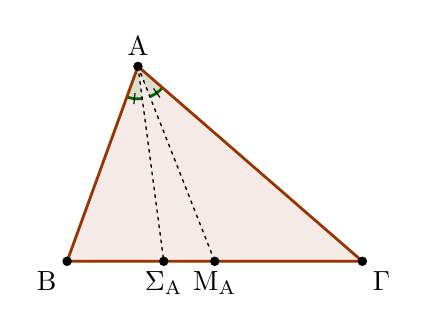
\begin{tikzpicture}[scale=.75]
\tkzSetUpLine[line width=1pt,color=black]
\tkzSetUpPoint[fill=black]

\tkzDefPoints{0/0/B,1.2/3.3/A,5/0/C}

\tkzDefTriangleCenter[in](A,B,C)
\tkzGetPoint{I}

\tkzDefMidPoint(B,C) \tkzGetPoint{MA}

\tkzDefTriangleCenter[symmedian](A,B,C)\tkzGetPoint{K}


\tkzInterLL(A,K)(B,C) \tkzGetPoint{SA}

\tkzFillPolygon[fill=ShapeClr,fill opacity=0.1](A,B,C)

\tkzFillAngles[fill=AngleClr,size=.55,fill opacity=0.1](B,A,SA MA,A,C)
\tkzMarkAngles[mark=|,mksize=2,line width=1pt,size=.55,color=AngleClr](B,A,SA MA,A,C)

\tkzDrawPolygon[color=ShapeClr](A,B,C)


\tkzDrawSegments[line width=0.5pt,color=black,dashed,dash pattern=on 1pt off 1.75pt](A,SA A,MA)

\tkzDrawPoints[size=3](A,B,C,SA,MA)
\tkzLabelPoint[above](A){$\rm A$}
\tkzLabelPoint[below left](B){$\rm B$}
\tkzLabelPoint[below right](C){$\rm \Gamma$}
\tkzLabelPoint[below](SA){$\rm \Sigma_A$}
\tkzLabelPoint[below](MA){$\rm M_A$}


\end{tikzpicture}

\end{document}
